% Options for packages loaded elsewhere
\PassOptionsToPackage{unicode}{hyperref}
\PassOptionsToPackage{hyphens}{url}
%
\documentclass[
  a4paper,
]{article}
\usepackage{amsmath,amssymb}
\usepackage{iftex}
\ifPDFTeX
  \usepackage[T1]{fontenc}
  \usepackage[utf8]{inputenc}
  \usepackage{textcomp} % provide euro and other symbols
\else % if luatex or xetex
  \usepackage{unicode-math} % this also loads fontspec
  \defaultfontfeatures{Scale=MatchLowercase}
  \defaultfontfeatures[\rmfamily]{Ligatures=TeX,Scale=1}
\fi
\usepackage{lmodern}
\ifPDFTeX\else
  % xetex/luatex font selection
  \setmainfont[]{Helvetica}
\fi
% Use upquote if available, for straight quotes in verbatim environments
\IfFileExists{upquote.sty}{\usepackage{upquote}}{}
\IfFileExists{microtype.sty}{% use microtype if available
  \usepackage[]{microtype}
  \UseMicrotypeSet[protrusion]{basicmath} % disable protrusion for tt fonts
}{}
\makeatletter
\@ifundefined{KOMAClassName}{% if non-KOMA class
  \IfFileExists{parskip.sty}{%
    \usepackage{parskip}
  }{% else
    \setlength{\parindent}{0pt}
    \setlength{\parskip}{6pt plus 2pt minus 1pt}}
}{% if KOMA class
  \KOMAoptions{parskip=half}}
\makeatother
\usepackage{xcolor}
\usepackage[margin=0.75in]{geometry}
\usepackage{graphicx}
\makeatletter
\def\maxwidth{\ifdim\Gin@nat@width>\linewidth\linewidth\else\Gin@nat@width\fi}
\def\maxheight{\ifdim\Gin@nat@height>\textheight\textheight\else\Gin@nat@height\fi}
\makeatother
% Scale images if necessary, so that they will not overflow the page
% margins by default, and it is still possible to overwrite the defaults
% using explicit options in \includegraphics[width, height, ...]{}
\setkeys{Gin}{width=\maxwidth,height=\maxheight,keepaspectratio}
% Set default figure placement to htbp
\makeatletter
\def\fps@figure{htbp}
\makeatother
\setlength{\emergencystretch}{3em} % prevent overfull lines
\providecommand{\tightlist}{%
  \setlength{\itemsep}{0pt}\setlength{\parskip}{0pt}}
\setcounter{secnumdepth}{-\maxdimen} % remove section numbering
\usepackage{titling}
\pretitle{\begin{flushleft}}
\posttitle{\end{flushleft}}
\usepackage{booktabs}
\usepackage{longtable}
\usepackage{float}
\floatplacement{figure}{H}
\usepackage{colortbl}
\usepackage{pdflscape}
\usepackage{tabu}
\usepackage{makecell}
\usepackage{xcolor}
\usepackage{soul}
\usepackage{caption}
\usepackage[singlelinecheck=false]{caption}
\usepackage[font={small,bf}]{caption}
\usepackage{multirow}
\usepackage{array}
\usepackage{lscape}
\newcommand{\blandscape}{\begin{landscape}}
\newcommand{\elandscape}{\end{landscape}}
\usepackage[dvipsnames]{xcolor}
\renewcommand{\footnotesize}{\tiny}
\usepackage{booktabs}
\usepackage{longtable}
\usepackage{array}
\usepackage{multirow}
\usepackage{wrapfig}
\usepackage{float}
\usepackage{colortbl}
\usepackage{pdflscape}
\usepackage{tabu}
\usepackage{threeparttable}
\usepackage{threeparttablex}
\usepackage[normalem]{ulem}
\usepackage{makecell}
\usepackage{xcolor}
\ifLuaTeX
  \usepackage{selnolig}  % disable illegal ligatures
\fi
\usepackage{bookmark}
\IfFileExists{xurl.sty}{\usepackage{xurl}}{} % add URL line breaks if available
\urlstyle{same}
\hypersetup{
  hidelinks,
  pdfcreator={LaTeX via pandoc}}

\title{\vspace{-1.5cm} \begin{LARGE} WGS Quality Control Report \end{LARGE}}
\author{}
\date{\vspace{-2.5em}}

\begin{document}
\maketitle

\normalsize Batch Name: 2024-07-23

\normalsize Experiment Name: 24ARS\_SATSCAN\_SALM\_LG77Y

\fontsize{7}{8}
\selectfont
\captionsetup[table]{labelformat=empty}
\renewcommand{\arraystretch}{1.2}

\begin{longtable}[t]{>{\centering\arraybackslash}p{1cm}>{\centering\arraybackslash}p{2cm}>{\centering\arraybackslash}p{1.5cm}>{\centering\arraybackslash}p{5.25cm}>{\centering\arraybackslash}p{5.25cm}}
\toprule
\multicolumn{1}{>{\centering\arraybackslash}p{1cm}}{\cellcolor[HTML]{D4D4D4}{\textbf{Isolate No.}}} & \multicolumn{1}{>{\centering\arraybackslash}p{2cm}}{\cellcolor[HTML]{D4D4D4}{\textbf{Sample ID}}} & \multicolumn{1}{>{\centering\arraybackslash}p{1.5cm}}{\cellcolor[HTML]{D4D4D4}{\textbf{Description}}} & \multicolumn{1}{>{\centering\arraybackslash}p{5.25cm}}{\cellcolor[HTML]{D4D4D4}{\textbf{ARSRL}}} & \multicolumn{1}{>{\centering\arraybackslash}p{5.25cm}}{\cellcolor[HTML]{D4D4D4}{\textbf{WGS}}}\\
\midrule
\cellcolor[HTML]{FFA77F}{1} & \cellcolor[HTML]{FFA77F}{22ARS\_BGH0179} & \cellcolor[HTML]{FFA77F}{NGO19} & \cellcolor[HTML]{FFA77F}{Haemophilus influenzae (x)} & \cellcolor[HTML]{FFA77F}{Neisseria gonorrhoeae}\\
\cellcolor[HTML]{FD7979}{2} & \cellcolor[HTML]{FD7979}{22ARS\_VSM0456} & \cellcolor[HTML]{FD7979}{NGO18} & \cellcolor[HTML]{FD7979}{Neisseria gonorrhoeae} & \cellcolor[HTML]{FD7979}{Neisseria gonorrhoeae}\\
3 & 23ARS\_BRH0005 & NGO20 & Neisseria gonorrhoeae & Neisseria gonorrhoeae\\
4 & 23ARS\_CVM0029 & NGO21 & Neisseria gonorrhoeae & Neisseria gonorrhoeae\\
5 & 23ARS\_CVM0039 & NGO22 & Neisseria gonorrhoeae & Neisseria gonorrhoeae\\
\addlinespace
6 & 24ARS\_BGH0040 & SAL75 & Salmonella species & Salmonella enterica\\
7 & 24ARS\_BGH0041 & SAL76 & Salmonella species & Salmonella enterica\\
\cellcolor[HTML]{FFA77F}{8} & \cellcolor[HTML]{FFA77F}{24ARS\_BGH0042} & \cellcolor[HTML]{FFA77F}{SAL77} & \cellcolor[HTML]{FFA77F}{Salmonella species} & \cellcolor[HTML]{FFA77F}{Salmonella enterica}\\
9 & 24ARS\_BGH0043 & SAL78 & Salmonella species & Salmonella enterica\\
\cellcolor[HTML]{FFA77F}{10} & \cellcolor[HTML]{FFA77F}{24ARS\_BGH0044} & \cellcolor[HTML]{FFA77F}{SAL79} & \cellcolor[HTML]{FFA77F}{Salmonella species} & \cellcolor[HTML]{FFA77F}{Salmonella enterica}\\
\addlinespace
11 & 24ARS\_BGH0045 & SAL80 & Salmonella Typhi & Salmonella typhi\\
12 & 24ARS\_BGH0071 & SAL81 & Salmonella species & Salmonella enterica\\
13 & 24ARS\_BGH0072 & SAL82 & Salmonella species & Salmonella enterica\\
14 & 24ARS\_STC\_CVM0010 & satscan & Pseudomonas aeruginosa & Pseudomonas aeruginosa\\
15 & 24ARS\_STC\_CVM0011 & satscan & Pseudomonas aeruginosa & Pseudomonas aeruginosa\\
\addlinespace
16 & 24ARS\_STC\_CVM0012 & satscan & Pseudomonas aeruginosa & Pseudomonas aeruginosa\\
17 & 24ARS\_STC\_CVM0013 & satscan & Pseudomonas aeruginosa & Pseudomonas aeruginosa\\
18 & 24ARS\_STC\_CVM0014 & satscan & Pseudomonas aeruginosa & Pseudomonas aeruginosa\\
19 & 24ARS\_STC\_CVM0015 & satscan & Pseudomonas aeruginosa & Pseudomonas aeruginosa\\
20 & 24ARS\_STC\_CVM0016 & satscan & Pseudomonas aeruginosa & Pseudomonas aeruginosa\\
\addlinespace
21 & 24ARS\_ZMC0002 & EMR156\_2 & Pseudomonas aeruginosa & Pseudomonas aeruginosa\\
\bottomrule
\multicolumn{5}{l}{\rule{0pt}{1em}\textit{Legend:} PASS   |   \colorbox{Peach}{WARNING}   |   \colorbox{Salmon}{FAILURE}   |   \textcolor{Blue}{EXCEEDS THRESHOLD METRIC/S}   |   (x) - NON-CONCORDANT   |}\\
\end{longtable}

\fontsize{7}{8}
\selectfont
\captionsetup[table]{labelformat=empty}
\renewcommand{\arraystretch}{1.2}

\begin{tabular}{>{\centering\arraybackslash}p{3cm}>{\centering\arraybackslash}p{3cm}>{\centering\arraybackslash}p{2cm}>{\centering\arraybackslash}p{7cm}}
\toprule
\multicolumn{4}{l}{\textbf{Sample excluded in the analysis}} \\
\cmidrule(l{3pt}r{3pt}){1-4}
\multicolumn{1}{>{\centering\arraybackslash}p{3cm}}{\cellcolor[HTML]{D4D4D4}{\textbf{Sample ID}}} & \multicolumn{1}{>{\centering\arraybackslash}p{3cm}}{\cellcolor[HTML]{D4D4D4}{\textbf{Description}}} & \multicolumn{1}{>{\centering\arraybackslash}p{2cm}}{\cellcolor[HTML]{D4D4D4}{\textbf{Index reads}}} & \multicolumn{1}{>{\centering\arraybackslash}p{7cm}}{\cellcolor[HTML]{D4D4D4}{\textbf{Remarks}}}\\
\midrule
24ARS\_NKI0054 & EMR160\_2 & 1.0832 & low read count\\
\bottomrule
\end{tabular}

\(\\\)

\fontsize{7}{8}
\selectfont
\captionsetup[table]{labelformat=empty}
\renewcommand{\arraystretch}{1.2}

\begin{ThreePartTable}
\begin{TableNotes}[para]
\item \textit{Legend:} 
\item PASS
\item   |  
\item \colorbox{Peach}{WARNING}
\item   |  
\item \colorbox{Salmon}{FAILURE}
\item   |  
\item \textcolor{Blue}{EXCEEDS THRESHOLD METRIC/S}
\item   |  
\end{TableNotes}
\begin{longtable}[t]{>{\centering\arraybackslash}p{1cm}>{\centering\arraybackslash}p{3cm}>{\centering\arraybackslash}p{2cm}>{\centering\arraybackslash}p{2cm}>{\centering\arraybackslash}p{2cm}>{\centering\arraybackslash}p{2cm}>{\centering\arraybackslash}p{2cm}}
\toprule
\multicolumn{1}{>{\centering\arraybackslash}p{1cm}}{\cellcolor[HTML]{D4D4D4}{\textbf{Isolate No.}}} & \multicolumn{1}{>{\centering\arraybackslash}p{3cm}}{\cellcolor[HTML]{D4D4D4}{\textbf{Sample ID}}} & \multicolumn{1}{>{\centering\arraybackslash}p{2cm}}{\cellcolor[HTML]{D4D4D4}{\textbf{Contamination}}} & \multicolumn{1}{>{\centering\arraybackslash}p{2cm}}{\cellcolor[HTML]{D4D4D4}{\textbf{Contigs}}} & \multicolumn{1}{>{\centering\arraybackslash}p{2cm}}{\cellcolor[HTML]{D4D4D4}{\textbf{GC Percent}}} & \multicolumn{1}{>{\centering\arraybackslash}p{2cm}}{\cellcolor[HTML]{D4D4D4}{\textbf{N50}}} & \multicolumn{1}{>{\centering\arraybackslash}p{2cm}}{\cellcolor[HTML]{D4D4D4}{\textbf{Total Length}}}\\
\midrule
\cellcolor[HTML]{FFA77F}{1} & \cellcolor[HTML]{FFA77F}{22ARS\_BGH0179} & \cellcolor[HTML]{FFA77F}{\textcolor{black}{0}} & \cellcolor[HTML]{FFA77F}{\textcolor{black}{85}} & \cellcolor[HTML]{FFA77F}{52.65} & \cellcolor[HTML]{FFA77F}{\textcolor{blue}{48631}} & \cellcolor[HTML]{FFA77F}{2071467}\\
\cellcolor[HTML]{FD7979}{2} & \cellcolor[HTML]{FD7979}{22ARS\_VSM0456} & \cellcolor[HTML]{FD7979}{\textcolor{black}{0}} & \cellcolor[HTML]{FD7979}{\textcolor{blue}{543}} & \cellcolor[HTML]{FD7979}{50.33} & \cellcolor[HTML]{FD7979}{\textcolor{black}{53055}} & \cellcolor[HTML]{FD7979}{2234632}\\
3 & 23ARS\_BRH0005 & \textcolor{black}{0} & \textcolor{black}{80} & 52.31 & \textcolor{black}{52897} & 2180777\\
4 & 23ARS\_CVM0029 & \textcolor{black}{0} & \textcolor{black}{79} & 52.57 & \textcolor{black}{58956} & 2118978\\
5 & 23ARS\_CVM0039 & \textcolor{black}{0} & \textcolor{black}{88} & 52.37 & \textcolor{black}{57741} & 2140058\\
\addlinespace
6 & 24ARS\_BGH0040 & \textcolor{black}{0} & \textcolor{black}{62} & 52.09 & \textcolor{black}{301434} & 4987437\\
7 & 24ARS\_BGH0041 & \textcolor{black}{0} & \textcolor{black}{25} & 52.11 & \textcolor{black}{742565} & 4766742\\
\cellcolor[HTML]{FFA77F}{8} & \cellcolor[HTML]{FFA77F}{* 24ARS\_BGH0042} & \cellcolor[HTML]{FFA77F}{\textcolor{black}{0}} & \cellcolor[HTML]{FFA77F}{\textcolor{black}{26}} & \cellcolor[HTML]{FFA77F}{52.16} & \cellcolor[HTML]{FFA77F}{\textcolor{black}{728119}} & \cellcolor[HTML]{FFA77F}{4760732}\\
9 & 24ARS\_BGH0043 & \textcolor{black}{0} & \textcolor{black}{58} & 52.13 & \textcolor{black}{217729} & 4963591\\
\cellcolor[HTML]{FFA77F}{10} & \cellcolor[HTML]{FFA77F}{* 24ARS\_BGH0044} & \cellcolor[HTML]{FFA77F}{\textcolor{black}{0}} & \cellcolor[HTML]{FFA77F}{\textcolor{black}{23}} & \cellcolor[HTML]{FFA77F}{52.03} & \cellcolor[HTML]{FFA77F}{\textcolor{black}{490148}} & \cellcolor[HTML]{FFA77F}{4773509}\\
\addlinespace
11 & 24ARS\_BGH0045 & \textcolor{black}{0} & \textcolor{black}{52} & 52.09 & \textcolor{black}{172613} & 4703271\\
12 & 24ARS\_BGH0071 & \textcolor{black}{0} & \textcolor{black}{56} & 52.13 & \textcolor{black}{299734} & 4975275\\
13 & 24ARS\_BGH0072 & \textcolor{black}{0} & \textcolor{black}{35} & 51.93 & \textcolor{black}{466584} & 5056128\\
14 & 24ARS\_STC\_CVM0010 & \textcolor{black}{0} & \textcolor{black}{82} & 66.37 & \textcolor{black}{214091} & 6392720\\
15 & 24ARS\_STC\_CVM0011 & \textcolor{black}{0} & \textcolor{black}{117} & 66.36 & \textcolor{black}{123460} & 6394288\\
\addlinespace
16 & 24ARS\_STC\_CVM0012 & \textcolor{black}{0} & \textcolor{black}{90} & 66.36 & \textcolor{black}{178858} & 6400798\\
17 & 24ARS\_STC\_CVM0013 & \textcolor{black}{0} & \textcolor{black}{88} & 66.36 & \textcolor{black}{214074} & 6404538\\
18 & 24ARS\_STC\_CVM0014 & \textcolor{black}{0} & \textcolor{black}{95} & 66.37 & \textcolor{black}{187092} & 6393505\\
19 & 24ARS\_STC\_CVM0015 & \textcolor{black}{0} & \textcolor{black}{51} & 66.42 & \textcolor{black}{436622} & 6353608\\
20 & 24ARS\_STC\_CVM0016 & \textcolor{black}{0} & \textcolor{black}{51} & 66.35 & \textcolor{black}{467470} & 6409137\\
\addlinespace
21 & 24ARS\_ZMC0002 & \textcolor{black}{0} & \textcolor{black}{43} & 66.46 & \textcolor{black}{430238} & 6331823\\
\bottomrule
\multicolumn{7}{l}{\rule{0pt}{1em}\textit{Note: } *Isolates were tagged with warning due to uncertain results of species identification using bactinspector.}\\
\insertTableNotes
\end{longtable}
\end{ThreePartTable}

\fontsize{7}{8}
\selectfont
\captionsetup[table]{labelformat=empty}
\renewcommand{\arraystretch}{1.2}

\begin{longtable}[t]{>{\centering\arraybackslash}p{2cm}>{\raggedright\arraybackslash}p{3cm}>{\centering\arraybackslash}p{11cm}}
\toprule
\multicolumn{3}{l}{\textbf{With Warning/s}} \\
\cmidrule(l{3pt}r{3pt}){1-3}
\multicolumn{1}{>{\centering\arraybackslash}p{2cm}}{\cellcolor[HTML]{D4D4D4}{\textbf{Isolate No.}}} & \multicolumn{1}{>{\centering\arraybackslash}p{3cm}}{\cellcolor[HTML]{D4D4D4}{\textbf{Sample ID}}} & \multicolumn{1}{>{\centering\arraybackslash}p{11cm}}{\cellcolor[HTML]{D4D4D4}{\textbf{Value with warning/s}}}\\
\midrule
\cellcolor{gray!10}{1} & \cellcolor{gray!10}{22ARS\_BGH0179} & \cellcolor{gray!10}{fastqc.1.Per.sequence.GC.content.metric\_value, fastqc.1.Sequence.Length.Distribution.metric\_value, fastqc.2.Per.sequence.GC.content.metric\_value, fastqc.2.Sequence.Length.Distribution.metric\_value}\\
8 & 24ARS\_BGH0042 & fastqc.1.Per.sequence.GC.content.metric\_value, fastqc.1.Sequence.Length.Distribution.metric\_value, fastqc.2.Per.sequence.GC.content.metric\_value, fastqc.2.Sequence.Length.Distribution.metric\_value\\
\cellcolor{gray!10}{10} & \cellcolor{gray!10}{24ARS\_BGH0044} & \cellcolor{gray!10}{fastqc.1.Per.sequence.GC.content.metric\_value, fastqc.1.Sequence.Length.Distribution.metric\_value, fastqc.2.Per.sequence.GC.content.metric\_value, fastqc.2.Sequence.Length.Distribution.metric\_value}\\
\bottomrule
\end{longtable}

\begin{longtable}[l]{cccccc}
\toprule
\multicolumn{6}{l}{\textbf{List of samples above/below QC threshold metrics}} \\
\cmidrule(l{3pt}r{3pt}){1-6}
\cellcolor[HTML]{D4D4D4}{\textbf{Sample ID}} & \cellcolor[HTML]{D4D4D4}{\textbf{Result}} & \cellcolor[HTML]{D4D4D4}{\textbf{Contamination}} & \cellcolor[HTML]{D4D4D4}{\textbf{Contigs}} & \cellcolor[HTML]{D4D4D4}{\textbf{N50}} & \cellcolor[HTML]{D4D4D4}{\textbf{Total Length}}\\
\midrule
22ARS\_VSM0456 & FAILURE & PASS & 543 & 53055 & 2234632\\
\bottomrule
\end{longtable}

\fontsize{7}{8}
\selectfont
\captionsetup[table]{labelformat=empty}
\renewcommand{\arraystretch}{1.2}

\begin{longtable}[l]{>{\raggedright\arraybackslash}p{8cm}c}
\toprule
\cellcolor[HTML]{D4D4D4}{\textbf{WGS\_ID}} & \cellcolor[HTML]{D4D4D4}{\textbf{Number}}\\
\midrule
Pseudomonas aeruginosa & 8\\
Salmonella enterica & 7\\
Neisseria gonorrhoeae & 5\\
Salmonella typhi & 1\\
\bottomrule
\end{longtable}

\begin{itemize}
\item
  \(\color{red}4\) distinct species were identified among
  \(\color{red}21\) isolates.
\item
  \(\color{red}80.95\) \% (n=17) of the isolates passed the QC, while
  \(\color{red}14.29\) \% (n=3) were tagged with warning.
\item
  Concordance between ARSRL and WGS species report was
  \(\color{red}95.24\) \%. \(\\\)
\end{itemize}

\subsubsection{GRAPHS}\label{graphs}

\fontsize{7}{8}
\selectfont
\captionsetup[table]{labelformat=empty}
\renewcommand{\arraystretch}{1.2}

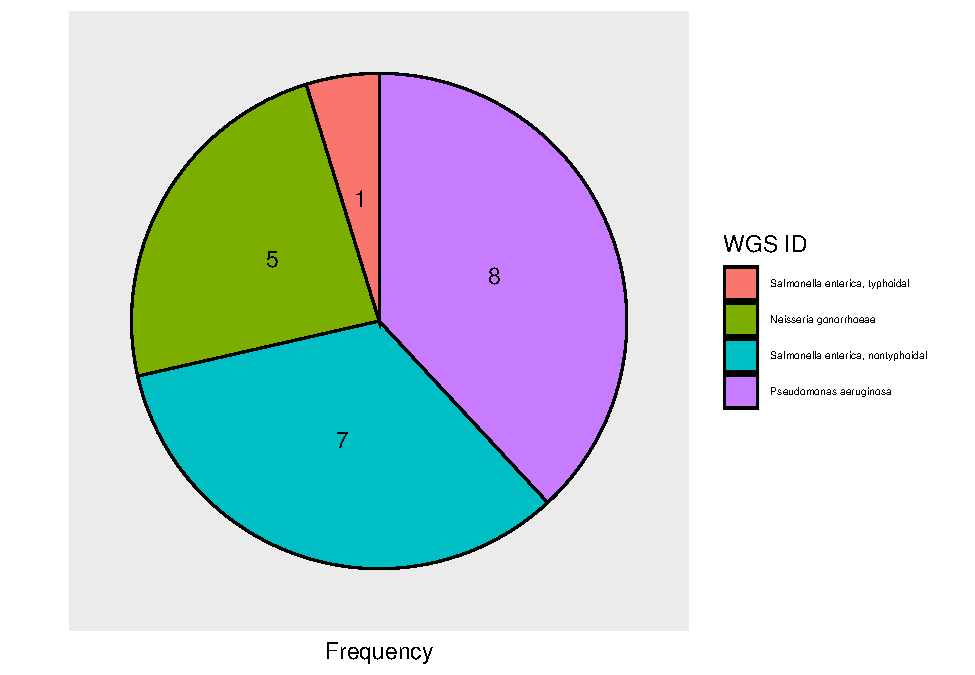
\includegraphics{qualifyr_report_2024-07-23_files/figure-latex/pie_chart-1.pdf}

\subsubsection{Result Classification}\label{result-classification}

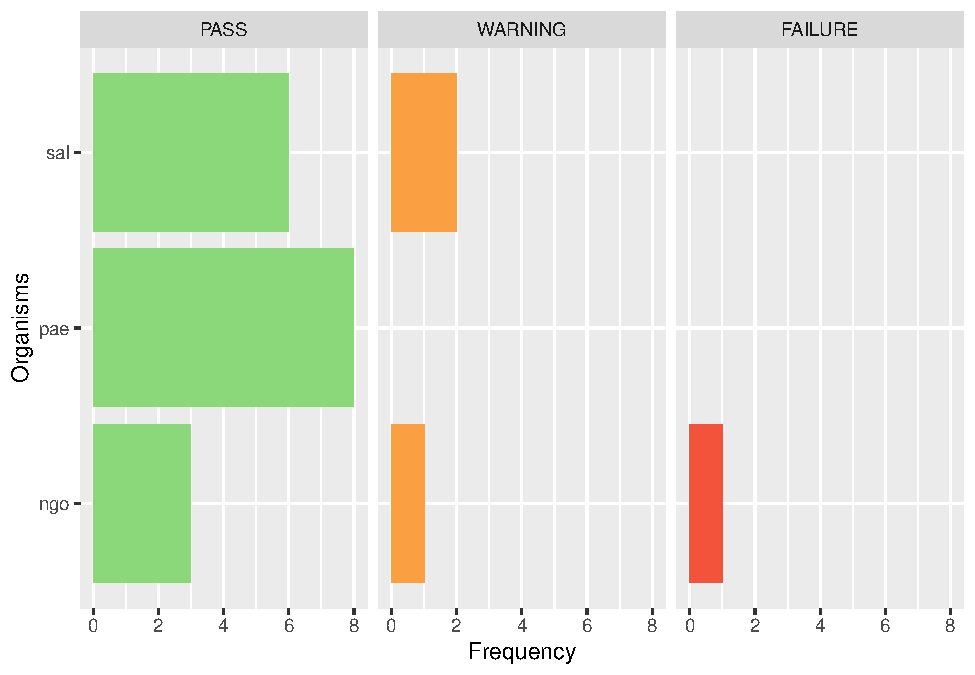
\includegraphics{qualifyr_report_2024-07-23_files/figure-latex/organism results-1.pdf}

\subsubsection{Number of contigs}\label{number-of-contigs}

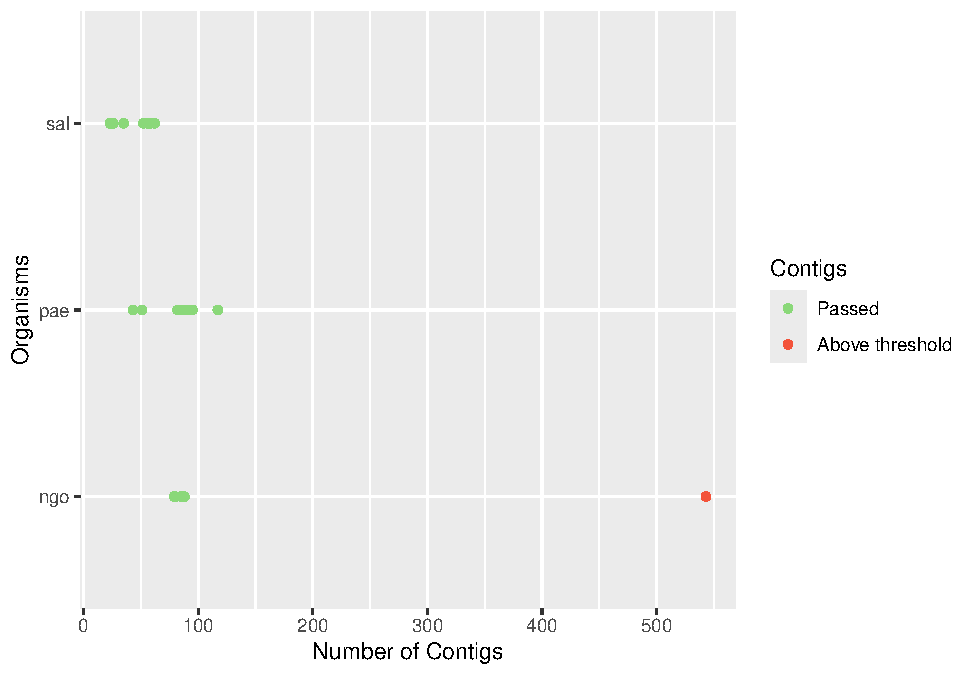
\includegraphics{qualifyr_report_2024-07-23_files/figure-latex/unnamed-chunk-1-1.pdf}

\subsubsection{N50 Value}\label{n50-value}

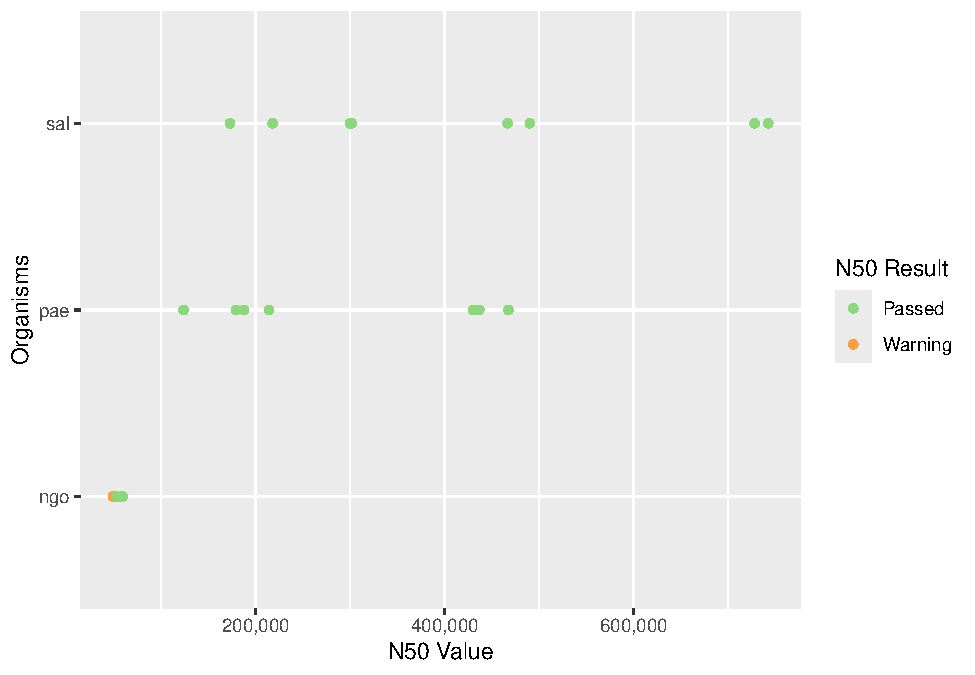
\includegraphics{qualifyr_report_2024-07-23_files/figure-latex/n50_result -1.pdf}

\subsubsection{Total Length}\label{total-length}

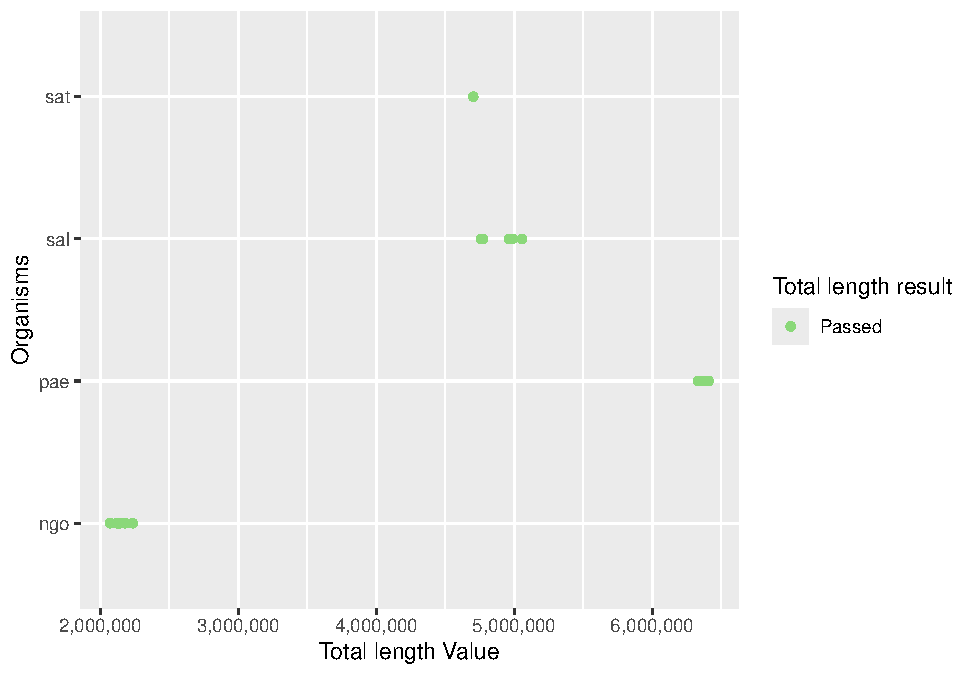
\includegraphics{qualifyr_report_2024-07-23_files/figure-latex/length_result -1.pdf}

\(\\\)

\subsubsection{RECOMMENDATION:}\label{recommendation}

\begin{longtable}[l]{>{\centering\arraybackslash}p{6cm}>{\centering\arraybackslash}p{4cm}>{\centering\arraybackslash}p{6cm}}
\toprule
\cellcolor[HTML]{D4D4D4}{\textbf{Sample ID}} & \cellcolor[HTML]{D4D4D4}{\textbf{Action}} & \cellcolor[HTML]{D4D4D4}{\textbf{Reason}}\\
\midrule
24ARS\_NKI0054 & Repeat testing & Low read count\\
22ARS\_VSM0456 & Repeat testing & QC failure (high contigs)\\
\bottomrule
\end{longtable}

\subsubsection{MLST RESULTS}\label{mlst-results}

\begin{longtable}[l]{>{\centering\arraybackslash}p{3cm}>{\centering\arraybackslash}p{3cm}>{\centering\arraybackslash}p{1cm}>{\centering\arraybackslash}p{1cm}>{\centering\arraybackslash}p{1cm}>{\centering\arraybackslash}p{1cm}>{\centering\arraybackslash}p{1cm}>{\centering\arraybackslash}p{1cm}>{\centering\arraybackslash}p{1cm}c}
\toprule
\cellcolor[HTML]{D4D4D4}{\textbf{sample\_id}} & \cellcolor[HTML]{D4D4D4}{\textbf{species}} & \cellcolor[HTML]{D4D4D4}{\textbf{MLST}} & \cellcolor[HTML]{D4D4D4}{\textbf{aroC.1.}} & \cellcolor[HTML]{D4D4D4}{\textbf{adk}} & \cellcolor[HTML]{D4D4D4}{\textbf{aroE}} & \cellcolor[HTML]{D4D4D4}{\textbf{fumC}} & \cellcolor[HTML]{D4D4D4}{\textbf{gdh}} & \cellcolor[HTML]{D4D4D4}{\textbf{pdhC}} & \cellcolor[HTML]{D4D4D4}{\textbf{pgm}}\\
\midrule
22ARS\_BGH0179 & Neisseria gonorrhoeae & 9364 & abcZ(435) & 39 & 67 & 158 & 148 & 71 & 65\\
22ARS\_VSM0456 & Neisseria gonorrhoeae & 7363 & abcZ(59) & 39 & 67 & 78 & 148 & 153 & 65\\
23ARS\_BRH0005 & Neisseria gonorrhoeae & 7823 & abcZ(435) & 39 & 170 & 111 & 148 & 153 & 65\\
23ARS\_CVM0029 & Neisseria gonorrhoeae & - & abcZ(59) & 39 & 170 & 78 & 149 & 71 & 65\\
23ARS\_CVM0039 & Neisseria gonorrhoeae & 10214 & abcZ(435) & 39 & 170 & 78 & 148 & 153 & 65\\
\bottomrule
\multicolumn{10}{l}{\rule{0pt}{1em}\textit{Legend: } (-) Not identified}\\
\end{longtable}

\begin{longtable}[l]{>{\centering\arraybackslash}p{3cm}>{\centering\arraybackslash}p{3cm}>{\centering\arraybackslash}p{1cm}>{\centering\arraybackslash}p{1cm}>{\centering\arraybackslash}p{1cm}>{\centering\arraybackslash}p{1cm}>{\centering\arraybackslash}p{1cm}>{\centering\arraybackslash}p{1cm}>{\centering\arraybackslash}p{1cm}c}
\toprule
\cellcolor[HTML]{D4D4D4}{\textbf{sample\_id}} & \cellcolor[HTML]{D4D4D4}{\textbf{species}} & \cellcolor[HTML]{D4D4D4}{\textbf{MLST}} & \cellcolor[HTML]{D4D4D4}{\textbf{aroC.1.}} & \cellcolor[HTML]{D4D4D4}{\textbf{adk}} & \cellcolor[HTML]{D4D4D4}{\textbf{aroE}} & \cellcolor[HTML]{D4D4D4}{\textbf{fumC}} & \cellcolor[HTML]{D4D4D4}{\textbf{gdh}} & \cellcolor[HTML]{D4D4D4}{\textbf{pdhC}} & \cellcolor[HTML]{D4D4D4}{\textbf{pgm}}\\
\midrule
24ARS\_BGH0040 & Salmonella enterica & 4431 & aroC(10) & 19 & 12 & 981 & 5 & 9 & 2\\
24ARS\_BGH0041 & Salmonella enterica & 64 & aroC(10) & 14 & 15 & 31 & 25 & 20 & 33\\
24ARS\_BGH0042 & Salmonella enterica & 684 & aroC(147) & 13 & 15 & 123 & 15 & 19 & 17\\
24ARS\_BGH0043 & Salmonella enterica & 32 & aroC(17) & 18 & 22 & 17 & 5 & 21 & 19\\
24ARS\_BGH0044 & Salmonella enterica & - & aroC(5,638) & 2 & 3 & 7 & 6 & 6 & 11\\
\addlinespace
24ARS\_BGH0071 & Salmonella enterica & 32 & aroC(17) & 18 & 22 & 17 & 5 & 21 & 19\\
24ARS\_BGH0072 & Salmonella enterica & 46 & aroC(10) & 7 & 21 & 12 & 15 & 12 & 12\\
\bottomrule
\multicolumn{10}{l}{\rule{0pt}{1em}\textit{Legend: } (-) Not identified}\\
\end{longtable}

\begin{longtable}[l]{>{\centering\arraybackslash}p{3cm}>{\centering\arraybackslash}p{3cm}>{\centering\arraybackslash}p{1cm}>{\centering\arraybackslash}p{1cm}>{\centering\arraybackslash}p{1cm}>{\centering\arraybackslash}p{1cm}>{\centering\arraybackslash}p{1cm}>{\centering\arraybackslash}p{1cm}>{\centering\arraybackslash}p{1cm}c}
\toprule
\cellcolor[HTML]{D4D4D4}{\textbf{sample\_id}} & \cellcolor[HTML]{D4D4D4}{\textbf{species}} & \cellcolor[HTML]{D4D4D4}{\textbf{MLST}} & \cellcolor[HTML]{D4D4D4}{\textbf{aroC.1.}} & \cellcolor[HTML]{D4D4D4}{\textbf{adk}} & \cellcolor[HTML]{D4D4D4}{\textbf{aroE}} & \cellcolor[HTML]{D4D4D4}{\textbf{fumC}} & \cellcolor[HTML]{D4D4D4}{\textbf{gdh}} & \cellcolor[HTML]{D4D4D4}{\textbf{pdhC}} & \cellcolor[HTML]{D4D4D4}{\textbf{pgm}}\\
\midrule
24ARS\_STC\_CVM0010 & Pseudomonas aeruginosa & 3654 & acsA(11) & 20 & 26 & 13 & 4 & 7 & 53\\
24ARS\_STC\_CVM0011 & Pseudomonas aeruginosa & 3654 & acsA(11) & 20 & 26 & 13 & 4 & 7 & 53\\
24ARS\_STC\_CVM0012 & Pseudomonas aeruginosa & 3654 & acsA(11) & 20 & 26 & 13 & 4 & 7 & 53\\
24ARS\_STC\_CVM0013 & Pseudomonas aeruginosa & 3654 & acsA(11) & 20 & 26 & 13 & 4 & 7 & 53\\
24ARS\_STC\_CVM0014 & Pseudomonas aeruginosa & 3654 & acsA(11) & 20 & 26 & 13 & 4 & 7 & 53\\
\addlinespace
24ARS\_STC\_CVM0015 & Pseudomonas aeruginosa & 500 & acsA(11) & 57 & 7 & 3 & 4 & 15 & 1\\
24ARS\_STC\_CVM0016 & Pseudomonas aeruginosa & - & acsA(19) & 5 & \textasciitilde{}1 & 61 & 55 & 12 & 3\\
24ARS\_ZMC0002 & Pseudomonas aeruginosa & 3014 & acsA(16) & 5 & 12 & 3 & 3 & 1 & 18\\
\bottomrule
\multicolumn{10}{l}{\rule{0pt}{1em}\textit{Legend: } (-) Not identified}\\
\end{longtable}

\begin{longtable}[l]{ccc}
\toprule
\cellcolor[HTML]{D4D4D4}{\textbf{sample\_id}} & \cellcolor[HTML]{D4D4D4}{\textbf{wgs\_id}} & \cellcolor[HTML]{D4D4D4}{\textbf{species}}\\
\midrule
24ARS\_BGH0045 & Salmonella typhi & No MLST result\\
\bottomrule
\end{longtable}

\subsubsection{MLST RESULTS SUMMARY:}\label{mlst-results-summary}

\begin{longtable}[l]{ll}
\toprule
\cellcolor[HTML]{D4D4D4}{\textbf{wgs\_id}} & \cellcolor[HTML]{D4D4D4}{\textbf{mlst\_count}}\\
\midrule
Neisseria gonorrhoeae & - (n= 1 ), 10214 (n= 1 ), 7363 (n= 1 ), 7823 (n= 1 ), 9364 (n= 1 )\\
Salmonella enterica & - (n= 1 ), 32 (n= 2 ), 4431 (n= 1 ), 46 (n= 1 ), 64 (n= 1 ), 684 (n= 1 )\\
Pseudomonas aeruginosa & - (n= 1 ), 3014 (n= 1 ), 3654 (n= 5 ), 500 (n= 1 )\\
\bottomrule
\multicolumn{2}{l}{\rule{0pt}{1em}\textit{Legend: } (-) Not identified}\\
\end{longtable}

\newpage
\begin{landscape}
\fontsize{7}{8}
\selectfont
\captionsetup[table]{labelformat=empty}
\renewcommand{\arraystretch}{1.2}

\subsubsection{AMR PREDICTION RESULTS}\label{amr-prediction-results}

\begin{tabular}{c>{\centering\arraybackslash}p{3cm}>{\centering\arraybackslash}p{3cm}>{\centering\arraybackslash}p{3cm}>{\centering\arraybackslash}p{3cm}}
\toprule
\multicolumn{5}{l}{\textbf{\textit{Neisseria gonorrhoeae}}} \\
\cmidrule(l{3pt}r{3pt}){1-5}
\cellcolor[HTML]{D4D4D4}{\textbf{sample\_id}} & \cellcolor[HTML]{D4D4D4}{\textbf{AMR BETA-LACTAM}} & \cellcolor[HTML]{D4D4D4}{\textbf{AMR EFFLUX}} & \cellcolor[HTML]{D4D4D4}{\textbf{AMR TETRACYCLINE}} & \cellcolor[HTML]{D4D4D4}{\textbf{STRESS EFFLUX}}\\
\midrule
22ARS\_BGH0179 & blaTEM-1 & mtrR, norM, farB, mtrC, mtrA & NA & mtrF\\
22ARS\_VSM0456 & blaTEM-1 & norM, mtrC, mtrR, mtrA, farB & tet(M) & mtrF\\
23ARS\_BRH0005 & blaTEM-1 & farB, norM, mtrC, mtrR, mtrA & tet(M) & mtrF\\
23ARS\_CVM0029 & blaTEM-135 & norM, mtrC, mtrR, mtrA, farB & NA & mtrF\\
23ARS\_CVM0039 & blaTEM-1 & norM, mtrC, mtrR, mtrA, farB & NA & mtrF\\
\bottomrule
\end{tabular}
\begin{table}[H]
\centering
\resizebox{\ifdim\width>\linewidth\linewidth\else\width\fi}{!}{
\begin{tabular}{c>{\centering\arraybackslash}p{3cm}>{\centering\arraybackslash}p{3cm}>{\centering\arraybackslash}p{3cm}>{\centering\arraybackslash}p{3cm}>{\centering\arraybackslash}p{3cm}>{\centering\arraybackslash}p{3cm}>{\centering\arraybackslash}p{3cm}>{\centering\arraybackslash}p{3cm}>{\centering\arraybackslash}p{3cm}>{\centering\arraybackslash}p{3cm}>{\centering\arraybackslash}p{3cm}>{\centering\arraybackslash}p{3cm}>{\centering\arraybackslash}p{3cm}>{\centering\arraybackslash}p{3cm}>{\centering\arraybackslash}p{3cm}>{\centering\arraybackslash}p{3cm}>{\centering\arraybackslash}p{3cm}>{\centering\arraybackslash}p{3cm}>{\centering\arraybackslash}p{3cm}>{\centering\arraybackslash}p{3cm}>{\centering\arraybackslash}p{3cm}>{\centering\arraybackslash}p{3cm}>{\centering\arraybackslash}p{3cm}>{\centering\arraybackslash}p{3cm}>{\centering\arraybackslash}p{3cm}>{\centering\arraybackslash}p{3cm}}
\toprule
\multicolumn{27}{l}{\textbf{\textit{Salmonella enterica}}} \\
\cmidrule(l{3pt}r{3pt}){1-27}
\cellcolor[HTML]{D4D4D4}{\textbf{sample\_id}} & \cellcolor[HTML]{D4D4D4}{\textbf{AMR APRAMYCIN/ GENTAMICIN/ TOBRAMYCIN}} & \cellcolor[HTML]{D4D4D4}{\textbf{AMR BETA-LACTAM}} & \cellcolor[HTML]{D4D4D4}{\textbf{AMR CEPHALOSPORIN}} & \cellcolor[HTML]{D4D4D4}{\textbf{AMR CHLORAMPHENICOL/ FLORFENICOL}} & \cellcolor[HTML]{D4D4D4}{\textbf{AMR EFFLUX}} & \cellcolor[HTML]{D4D4D4}{\textbf{AMR HYGROMYCIN}} & \cellcolor[HTML]{D4D4D4}{\textbf{AMR KANAMYCIN}} & \cellcolor[HTML]{D4D4D4}{\textbf{AMR LINCOSAMIDE}} & \cellcolor[HTML]{D4D4D4}{\textbf{AMR QUINOLONE}} & \cellcolor[HTML]{D4D4D4}{\textbf{AMR STREPTOMYCIN}} & \cellcolor[HTML]{D4D4D4}{\textbf{AMR SULFONAMIDE}} & \cellcolor[HTML]{D4D4D4}{\textbf{AMR TETRACYCLINE}} & \cellcolor[HTML]{D4D4D4}{\textbf{AMR TRIMETHOPRIM}} & \cellcolor[HTML]{D4D4D4}{\textbf{STRESS ARSENATE}} & \cellcolor[HTML]{D4D4D4}{\textbf{STRESS ARSENIC}} & \cellcolor[HTML]{D4D4D4}{\textbf{STRESS ARSENITE}} & \cellcolor[HTML]{D4D4D4}{\textbf{STRESS COPPER}} & \cellcolor[HTML]{D4D4D4}{\textbf{STRESS COPPER/ GOLD}} & \cellcolor[HTML]{D4D4D4}{\textbf{STRESS COPPER/ SILVER}} & \cellcolor[HTML]{D4D4D4}{\textbf{STRESS GOLD}} & \cellcolor[HTML]{D4D4D4}{\textbf{STRESS MERCURY}} & \cellcolor[HTML]{D4D4D4}{\textbf{STRESS NA}} & \cellcolor[HTML]{D4D4D4}{\textbf{STRESS ORGANOMERCURY}} & \cellcolor[HTML]{D4D4D4}{\textbf{STRESS QUATERNARY AMMONIUM}} & \cellcolor[HTML]{D4D4D4}{\textbf{STRESS SILVER}} & \cellcolor[HTML]{D4D4D4}{\textbf{VIRULENCE NA}}\\
\midrule
24ARS\_BGH0040 & aac(3)-IVa & blaTEM-1 & NA & floR & mdsA, mdsB & NA & NA & NA & NA & aph(6)-Id, aph(3'')-Ib & sul2 & tet(B) & NA & arsC & arsR & arsB, arsA, arsD & pcoS, pcoR, pcoD, pcoC, pcoA & golT & silB, silF, silC, silR, silS, silA & golS & merP, merT, merR & fieF & merC & NA & silE, silP & iroB, iroC, sinH, sodC1\\
24ARS\_BGH0041 & NA & NA & blaDHA-1 & floR & mdsA, mdsB & NA & NA & lnu(F) & qnrB4 & aph(6)-Id, aph(3'')-Ib, aadA2 & sul1, sul2 & tet(A) & dfrA23 & NA & NA & NA & NA & golT & NA & golS & NA & fieF & NA & qacE & NA & sinH, iroB, iroC\\
24ARS\_BGH0042 & NA & NA & NA & NA & mdsA, mdsB & NA & NA & NA & NA & NA & NA & NA & NA & NA & NA & NA & NA & golT & NA & golS & NA & fieF & NA & NA & NA & sinH, sodC1, iroC, iroB\\
24ARS\_BGH0043 & aac(3)-IVa & NA & blaCTX-M-65 & NA & mdsA, mdsB & aph(4)-Ia & aph(3')-Ia & NA & NA & aadA1 & sul1 & tet(A) & NA & NA & arsR & NA & NA & golT & NA & golS & merP, merT, merR & fieF & merC & qacEdelta1 & NA & sinH, iroB, iroC, ybtP, ybtQ\\
24ARS\_BGH0044 & NA & NA & NA & NA & mdsB, mdsA & NA & NA & NA & NA & NA & NA & NA & NA & NA & NA & NA & NA & golT & NA & golS & NA & fieF & NA & NA & NA & sinH, sodC1, iroC, iroB\\
\addlinespace
24ARS\_BGH0071 & aac(3)-IVa & NA & blaCTX-M-65 & floR & mdsA, mdsB & aph(4)-Ia & NA & NA & NA & aadA1 & sul1 & tet(A) & dfrA14 & NA & arsR & NA & NA & golT & NA & golS & merP, merT, merR & fieF & merC & qacEdelta1 & NA & sinH, ybtP, ybtQ, iroB, iroC\\
24ARS\_BGH0072 & NA & blaTEM-1 & NA & floR & mdsA, mdsB & NA & NA & lnu(F) & NA & aadA2, aph(6)-Id, aph(3'')-Ib & sul1, sul2 & tet(D) & NA & NA & NA & NA & NA & golT & NA & golS & NA & fieF & NA & qacE & NA & iroB, iroC, sinH\\
\bottomrule
\end{tabular}}
\end{table}

\begin{tabular}{c>{\centering\arraybackslash}p{3cm}>{\centering\arraybackslash}p{3cm}}
\toprule
\multicolumn{3}{l}{\textbf{\textit{Salmonella typhi}}} \\
\cmidrule(l{3pt}r{3pt}){1-3}
\cellcolor[HTML]{D4D4D4}{\textbf{sample\_id}} & \cellcolor[HTML]{D4D4D4}{\textbf{STRESS NA}} & \cellcolor[HTML]{D4D4D4}{\textbf{VIRULENCE NA}}\\
\midrule
24ARS\_BGH0045 & fieF & iroB, sinH, iroC, cdtB\\
\bottomrule
\end{tabular}
\begin{table}[H]
\centering
\resizebox{\ifdim\width>\linewidth\linewidth\else\width\fi}{!}{
\begin{tabular}{c>{\centering\arraybackslash}p{3cm}>{\centering\arraybackslash}p{3cm}>{\centering\arraybackslash}p{3cm}>{\centering\arraybackslash}p{3cm}>{\centering\arraybackslash}p{3cm}>{\centering\arraybackslash}p{3cm}}
\toprule
\multicolumn{7}{l}{\textbf{\textit{Pseudomonas aeruginosa}}} \\
\cmidrule(l{3pt}r{3pt}){1-7}
\cellcolor[HTML]{D4D4D4}{\textbf{sample\_id}} & \cellcolor[HTML]{D4D4D4}{\textbf{AMR BETA-LACTAM}} & \cellcolor[HTML]{D4D4D4}{\textbf{AMR CEPHALOSPORIN}} & \cellcolor[HTML]{D4D4D4}{\textbf{AMR CHLORAMPHENICOL}} & \cellcolor[HTML]{D4D4D4}{\textbf{AMR EFFLUX}} & \cellcolor[HTML]{D4D4D4}{\textbf{AMR FOSFOMYCIN}} & \cellcolor[HTML]{D4D4D4}{\textbf{AMR KANAMYCIN}}\\
\midrule
24ARS\_STC\_CVM0010 & blaOXA-1127 & blaPDC-5 & catB7 & mexA, mexE, mexX & fosA & aph(3')-IIb\\
24ARS\_STC\_CVM0011 & blaOXA-1127 & blaPDC-5 & catB7 & mexA, mexX, mexE & fosA & aph(3')-IIb\\
24ARS\_STC\_CVM0012 & blaOXA-1127 & blaPDC-5 & catB7 & mexA, mexX, mexE & fosA & aph(3')-IIb\\
24ARS\_STC\_CVM0013 & blaOXA-1127 & blaPDC-5 & catB7 & mexA, mexE, mexX & fosA & aph(3')-IIb\\
24ARS\_STC\_CVM0014 & blaOXA-1127 & blaPDC-5 & catB7 & mexA, mexE, mexX & fosA & aph(3')-IIb\\
\addlinespace
24ARS\_STC\_CVM0015 & blaOXA-486 & blaPDC-1 & catB7 & mexA, mexE, mexX & fosA & aph(3')-IIb\\
24ARS\_STC\_CVM0016 & blaOXA-486 & blaPDC-5 & catB7 & mexA, mexE, mexX & fosA & aph(3')-IIb\\
24ARS\_ZMC0002 & blaOXA-1023 & blaPDC-3 & catB7 & mexA, mexE, mexX & fosA & aph(3')-IIb\\
\bottomrule
\end{tabular}}
\end{table}

\end{landscape}

\end{document}
